
\part{Method}

Based on the categorization of planning algorithms by Bitar\cite{bitar}, the algorithms shown in Figure \ref{fig:algorithms} is considered for the path planner.

\begin{figure}[h]
    \centering
    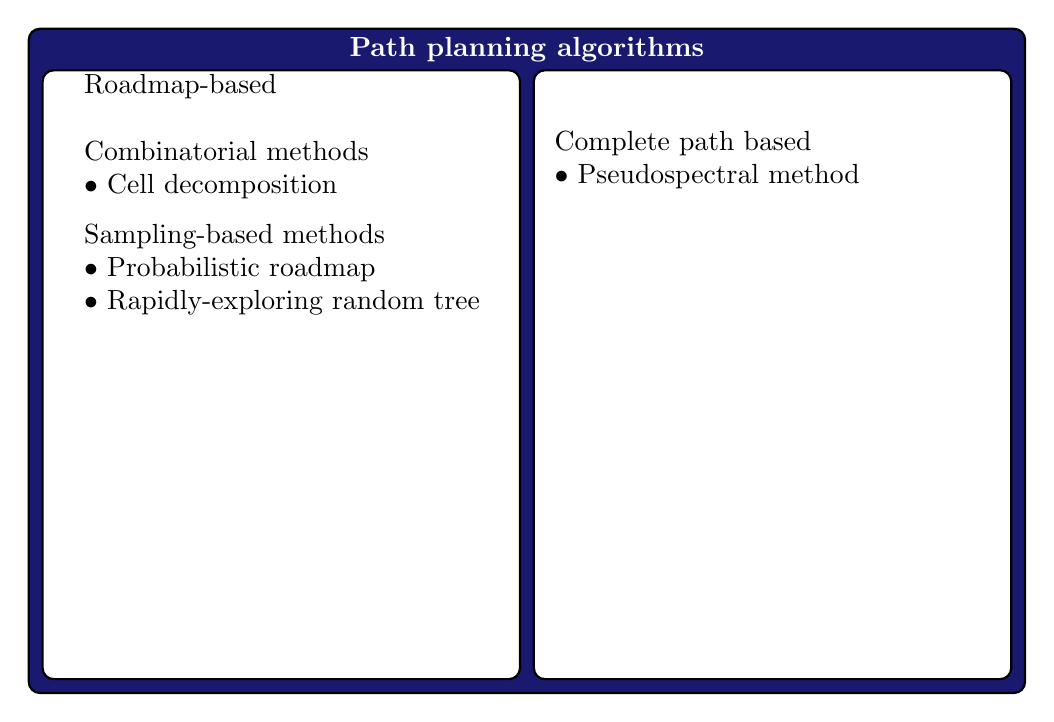
\begin{tikzpicture}[x=1em,y=1em]

	\tikzstyle{block} = [rectangle, draw, thick, fill=white,
    		text centered, rounded corners]
	\tikzstyle{block_marked} = [block, fill=MidnightBlue, text=white, font=\bfseries]
	\tikzstyle{text_marked} = [text=white, font=\bfseries]

    \node [block_marked, minimum height=24em, minimum width=36em] (main) {};
    \node [block, minimum height=22em, minimum width=17.25em] at (-8.875,-0.5) {};
    \node [block, minimum height=22em, minimum width=17.25em] at (8.875,-0.5) {};
    
    \node[text_marked] at (0,11.25) {Path planning algorithms};
   % \node[text width=10em] at (-8,0) {Roadmap-based };
	 \node[text width=15em] at (-8.5,6) {
    		Roadmap-based \\
    		 \bigskip
    		Combinatorial methods \\
  		$\bullet$ Cell decomposition \\
  		\medskip
  		Sampling-based methods \\
  		$\bullet$ Probabilistic roadmap \\
  		$\bullet$ Rapidly-exploring random tree \\
  		
	};
	\node[text width=15em] at (8.5,7.25) {
    		Complete path based \\
  		$\bullet$ Pseudospectral method
	};
   
\end{tikzpicture}
    \caption{Categorization of planning algorithms by Bitar\cite{bitar}}
    \label{fig:algorithms}
\end{figure}

\section{Algorithms}
\subsection{Algorithm A: Rapidly-Exploring Random Tree}

Rapidly-Exploring Random Tree (RRT) with bias and smoothing. Based on hybrid COLAV by Einvald Serigstad.

\begin{algorithm}
\caption{Rapidly-Exploring Random Tree}\label{euclid}
\begin{algorithmic}[1]
\Procedure{$\textsc{generate\_tree}(\boldsymbol{x}_{init})$}{}
\State $\boldsymbol{\Upsilon} \gets \text{init\_tree}(\boldsymbol{x}_{init})$
\Repeat
\State $\boldsymbol{p}_{new} \gets \textsc{random\_waypoint()}$

\For {$(n_{near}, \boldsymbol{p}_{near}, \boldsymbol{x}_{near}) \gets \textsc{nearest\_nodes}(\boldsymbol{\Upsilon}, \boldsymbol{p}_{new})$}

\State $(traj,\boldsymbol{x}_{new}) \gets \textsc{generate\_trajectory}(\boldsymbol{x}_{near}, \boldsymbol{p}_{new})$
\If{$\textsc{collision\_free}(traj)$}
	\State $\boldsymbol{\Upsilon} \gets \text{add\_node}(n_{new}, \boldsymbol{p}_{new}, \boldsymbol{x}_{new}, traj)$
	\State \textbf{break}
\EndIf
\EndFor

\Until{$\textsc{stop\_condition}(\boldsymbol{\Upsilon})$}\
\State \Return{$\boldsymbol{\Upsilon}$}
\EndProcedure

\end{algorithmic}
\end{algorithm}


$\textsc{nearest\_nodes}(\boldsymbol{\Upsilon}, \boldsymbol{p}_{new})$ returns a list of all nodes in $\boldsymbol{\Upsilon}$ sorted by the cost of connecting $\boldsymbol{p}_{new}$ to a node given by
\begin{equation}
	c() =  ||
\end{equation}

\subsection{Algorithm B: Pseudospectral method}
Based on Glenn Bitar's article on "Energy-Optimized Path Planning for Autonomous Ferries"

\subsection{Algorithm C: Cell decomposition}
Cell decomposition with A* search.

\subsection{Algorithm D: Visibility graph}
An alternative, but not most important.




\section{Test framework}
Algorithms are tested by simulating path-following and ship dynamics in different scenarios, and then comparing performance metrics.


\subsection{Scenarios}

\begin{enumerate}
	\item Ferry crossing, crossing of fjord. The end of the mission is in the horizon.
	\item Coastal area with moving boats. Dynamic.
	\item Open ocean with moving ships. Mission is approximated by a direction because the end is so far away.
\end{enumerate}


\subsection{Objective}

\subsubsection{COLREGS}
The International Regulations for Preventing Collisions at Sea from 1972. These regulations are made for ships controlled by humans, and autonomous ships must also be aware of these rules, since an autonomous ship will not be alone in the sea.

\subsubsection{Performance metrics}
Measure performance of the methods in terms of 
\begin{itemize}
	\item Computational time
	\item Travel time. Problem: Uses unrealistic actuation or not energy-efficient actuation.
	\item Energy efficiency. Using less actuation. Problem: Best solution is doing nothing.
	\item Robustness. Will it choose the faster path through reefs (vulnerable to deviations), or the safer path around? If choosing the reefs, will it slow down to minimize the chance of collision? The performance metric should take into consideration that the ship may not follow the path perfectly.
\end{itemize}

